%! Author = Yannis Teissier \& Wolodia Zdetovetzky
%! Date = 04/2023
\documentclass{article}

\usepackage[utf8]{inputenc}
\usepackage[T1]{fontenc}
\usepackage{amsmath}
\usepackage{listings}
\usepackage{graphicx}
\usepackage{hyperref}
\usepackage{lstdoc}
\inputencoding{utf8}

\title{Massive data processing \\ with the Unsplash dataset}
\author{Yannis TEISSIER \& Wolodia ZDETOVETZKY}
\date{03/2023}


\begin{document}

    \maketitle
    \tableofcontents
    \newpage


    \section{Objectives}\label{sec:objectives}

    In this project, we aimed to develop a comprehensive image recommendation system based on the Unsplash image dataset, taking into account user preferences.
    The following steps explain the objectives we pursued in order to achieve this goal.

    \textbf{Data Collection}\\
    Our first objective was to efficiently collect and process the large volume of data available in the Unsplash image dataset.
    We achieved this by parallelling the download process across multiple processes to enhance performance.

    \textbf{Data Annotation}\\
    To enrich the dataset, we aimed to automatically annotate the images with relevant metadata.
    This involved using Facebook's Detr AI for image recognition, which allowed us to generate descriptive tags for each image.

    \textbf{Dominant Color Extraction}\\
    We aimed to identify the four most dominant colors in each image to further enrich the metadata.
    To achieve this, we employed the K-means clustering algorithm,
    which allowed us to determine the most representative colors in each image effectively.

    \textbf{Data Visualization}\\
    We sought to expand the data visualization capabilities to align with the most relevant metadata obtained during the annotation and color extraction processes.
    This objective aimed to facilitate a better understanding of the dataset characteristics and user preferences.

    \textbf{Recommendation System Development}\\
    A central objective of this project was the development of an effective image recommendation system.
    We explored various techniques, such as Euclidean distance, cosine similarity, and Reinforcement Learning, to identify the best approach for providing personalized image recommendations to users.

    \textbf{Web Interface Implementation}\\
    The creation of a user-friendly web interface was our objective, enabling users to define their profiles and receive image recommendations.

    In annexe, you will find the~\hyperref[subsec:target_architecture]{\nameref{subsec:target_architecture}} proposed by the initial subject, followed by the~\hyperref[subsec:actual_architecture]{\nameref{subsec:actual_architecture}} of the project.

    \newpage


    \section{Data}\label{sec:data}

    \subsection{Data Source}\label{subsec:data_source}
    For our data source, we decided to use the Unsplash dataset (\url{https://github.com/unsplash/datasets}).
    This dataset consists of over 250,000 images contributed by photographers with diverse contexts, subjects, and use cases.

    \subsection{Licensing}\label{subsec:licensing}
    As stated on their website, Unsplash grants a worldwide, irrevocable, and non-exclusive copyright license for
    downloading, copying, modifying, distributing, reproducing, displaying, and using Unsplash photos free of charge, including for commercial purposes, without requiring additional permission from the photographer or Unsplash.
    This license does not include the right to compile Unsplash photos to replicate a similar or competing service.
    It is also worth mentioning that attributing credit is appreciated to help grow their community.
    Regarding the datasets, the Lite version is available for both commercial and non-commercial use.
    However, the complete dataset is intended for non-commercial use only.

    \subsection{Data Size}\label{subsec:data_size}
    In terms of data dimensions, Unsplash offers more than 3 million curated images, thanks to a community of nearly 300,000 professional and amateur photographers.
    The Lite dataset contains 25k nature-themed photos, 25k keywords, and 1 million searches.
    The complete dataset contains over 3 million high-quality photos, 5 million keywords, and more than 250 million searches.

    \subsection{Stored Information}\label{subsec:stored_infos}
    We store all the extracted metadata for the images in our database, along with the generated tags and dominant colors for each image.
    The following is a list of the stored fields: filename, Make, Model, Software, BitsPerSample, ImageWidth, ImageHeight, ImageDescription, Orientation, Copyright, DateTime, DateTimeOriginal, DateTimeDigitized, SubSecTimeOriginal, ExposureTime, FNumber, ExposureProgram, ISOSpeedRatings, SubjectDistance, ExposureBiasValue, Flash, FlashReturnedLight, FlashMode, MeteringMode, FocalLength, FocalLengthIn35mm, Latitude, LatitudeDegrees, LatitudeMinutes, LatitudeSeconds, LatitudeDirection, Longitude, LongitudeDegrees, LongitudeMinutes, LongitudeSeconds, LongitudeDirection, Altitude, DOP, FocalLengthMin, FocalLengthMax, FStopMin, FStopMax, LensMake, LensModel, FocalPlaneXResolution, FocalPlaneYResolution, tags, dominant\_color.
    In addition to the metadata, we store the images themselves in a Minio database.
    Minio is a high-performance, secure, and scalable object storage solution.

    \subsection{User preferences}\label{subsec:user_pref}
    Through the web interface, we collect user data to provide personalized image recommendations.
    Users are asked to fill in various fields, such as their favorite color using a color picker (which yields a hexadecimal code),
    desired image dimensions (height and width), orientation (landscape or portrait),
    tags representing the elements they wish to visualize (up to a maximum of 5), and the preferred camera make.
    This information is then used to generate recommendations that align with the user's preferences.


    \section{Data exploration}\label{sec:exploration}

    \subsection{Used models}\label{subsec:models}
    Throughout this project, various models and libraries were employed, both integrated and standalone:

    \begin{itemize}
        \item \textbf{Spacy}: A Python NLP library used for text processing and tag generation.\\It enables similarity association between tags and their categorization.
        \item \textbf{Mini-batch K-means}: A clustering algorithm used for dominant color generation.\\To enhance the algorithm's efficiency, we chose to reduce the image size to 200x200 pixels.\\Additionally, Mini-batch K-means was preferred over the standard K-means algorithm due to its faster performance.
        \item \textbf{Detr}: An image recognition model used for tag generation.\\Prior to selecting Detr, several attempts were made with other models, such as YoloV3, Google Owlvit, and Detr.\\Google Owlvit and YoloV3 were ultimately rejected due to their high processing time and download requirements.\\Initially, we used Detr with 300 parameters, but for similar reasons, we switched to the 50-parameter version, offering the best balance between processing and download time and accuracy.
        \item \textbf{Reinforcement Learning}: We have also tried to use Reinforcement Learning to improve the recommendation system using SB3.\\Stable Baselines3 (SB3) is a Python library implementing state-of-the-art Reinforcement Learning (RL) algorithms, aiming to facilitate their use in research and development projects.\\One such algorithm is the Deep Q-Network (DQN), designed for environments with large state and action spaces.\\In this project, the goal was to train an RL model to determine the Euclidean distance between a user's preferences and image vectors in a dataset using DQN.\\However, the reward system was found to be insufficiently relevant and time-consuming, hindering the agent's learning process.\\The problem might have been better addressed using supervised or unsupervised learning approaches instead.\\Consequently, while SB3 and DQN are powerful tools for RL, their effectiveness depends on the quality of the reward system and the suitability of applying RL to the problem at hand.
    \end{itemize}

    \subsection{Metrics}\label{subsec:metrics}
    \begin{itemize}
        \item \textbf{Spacy}: The \("\)en\_core\_web\_md\("\) model, version 3.5.0, is a medium-sized (40 MB) English natural language processing model developed by Explosion and distributed under the MIT license.\\Optimized for CPU performance, it incorporates multiple components to perform various NLP tasks, such as tokenization, part-of-speech tagging, named entity recognition, and lemmatisation.\\The model is pretrained on web-based text data and includes 300-dimensional word vectors.\\Its performance is evaluated in terms of accuracy, recall, and F-score, with a tokenization accuracy of 1.00 and an F-score of 0.85 for named entity recognition.\\This model was chosen over other models offered by spaCy as it provided the best balance between size and performance, given the resources available for our project.
        \item \textbf{Mini-batch K-means}: According to the performance report between K-Means and Mini-batch K-Means available \href{https://upcommons.upc.edu/bitstream/handle/2117/23414/R13-8.pdf}{here}, KMeans generally produces a higher level of cluster coherence, as indicated by smaller intra-cluster distances and higher silhouette scores.\\However, MiniBatchKMeans has a significant advantage in terms of computational efficiency, with shorter processing times and lower memory requirements.\\As such, we decided to use MiniBatchKMeans to promote the processing speed of our model.
        \item \textbf{Detr}: Concerning Detr, we use a list of 91 different objects on which the model is trained.\\In particular, it has been trained on COCO 2017 object detection, a dataset consisting of 118k/5k annotated images for training/validation respectively.\\This model achieves an AP (average precision) of 42.0 on COCO 2017 validation.\\Here is the list of recognized objects:\\N/A, person, traffic light, fire hydrant, street sign, stop sign, parking meter, bench, bird, cat, dog, horse, bicycle, sheep, cow, elephant, bear, zebra, giraffe, hat, backpack, umbrella, shoe, car, eye glasses, handbag, tie, suitcase, frisbee, skis, snowboard, sports ball, kite, baseball bat, motorcycle, baseball glove, skateboard, surfboard, tennis racket, bottle, plate, wine glass, cup, fork, knife, airplane, spoon, bowl, banana, apple, sandwich, orange, broccoli, carrot, hot dog, pizza, bus, donut, cake, chair, couch, potted plant, bed, mirror, dining table, window, desk, train, toilet, door, tv, laptop, mouse, remote, keyboard, cell phone, microwave, oven, truck, toaster, sink, refrigerator, blender, book, clock, vase, scissors, teddy bear, hair drier, boat, toothbrush.
        \item \textbf{Visualisation}: The collection of all these data also allowed us to visualize them and to obtain an overall vision of them through the graphs.\\We note in particular that the majority of the images were taken between in 2019 by Canon cameras and enormously in the USA. They were taken in large majority between 0 and 2000m of altitude, often represents people. The colors are mostly black, shades of gray and green.\\You will find some of these representations in Appendix ~~hyperref[subsec:Graphs]{\nameref{subsec:graphs}}.
    \end{itemize}

    Thus, in general, these metrics allowed us to guide our choice of models.
    We were able to decide to favor speed of processing and size of models while balancing this with accuracy of results.
    This allows us to offer an optimal user experience, while maintaining a certain accuracy of results.


    \section{Self-assessment}\label{sec:self_assessment}
    In terms of self-assessment, we have exceeded expectations for most of our objectives.
    We successfully implemented a functional recommendation system, complete with a web interface and the most efficient possible databases for storing the data we use.
    The numerous technologies we have employed and attempted to integrate sometimes involve advanced techniques, always with the aim of providing the most effective solution possible.
    This is demonstrated in the addition of extra constraints, such as EXIF extraction, automatic image tagging, and the automation of generating all of our metrics, among others.
    This comprehensive approach makes our project more complete and scientifically interesting.
    Therefore, we believe that our work stands among the higher tier of projects in this course.
    Consequently, if a grading were to be assigned, we think our project would be placed in the same high range.


    \section{Remarks}\label{sec:remarks}

    \subsection{Practical Sessions}\label{subsec:sessions}
    Regarding the practical sessions, we were quite disappointed not to have had more time dedicated to the project's realization.
    Indeed, the project is complex, requires diverse skills, and, for the most part, is entirely new.
    Similarly, the boundary between the expected outcome in the project's presentation document and the actual expected outcome is somewhat unclear.
    As a result, the project's size has caused concern among the class members, and this has affected the completion of the practical session exercises.
    The biggest issue, however, remains the working conditions in the computer lab.
    Due to the weak internet connection, inadequate rooms, and the absence of a second screen, the project's progress has been significantly slowed down.
    We were not fully equipped to successfully carry out the project, especially when it came to downloading large volumes of data.
    Nevertheless, we appreciated the variety of speakers, particularly the course presented by Mr. Martin.

    \subsection{Exercises}\label{subsec:exercises}
    Regarding the exercises, we, unfortunately, could not complete them in their entirety.
    Indeed, the project's size forced us to focus directly on its realization.

    \subsection{Improvements}\label{subsec:improvements}
    As for improvements, we have already mentioned the recurrent internet connection problems in the CPE rooms.
    One solution would be to directly address this issue or, more simply, to offer remote work sessions.
    Regarding the project, we would have liked to have more time to complete the exercises and the project, as the lack of time prevented us from achieving some of the objectives.
    The project being quite substantial, it would have been preferable to reduce its size and clearly define the expected goals.
    Additionally, a thorough review and correction of the project's implementation would have been a plus.


    \section{Conclusion}\label{sec:conclusion}

    In conclusion, we have successfully developed a comprehensive image recommendation system based on the Unsplash dataset, taking into account user preferences.
    Through our work, we achieved multiple objectives, including efficient data collection, automatic data annotation, dominant color extraction, data visualization enhancement, and the implementation of a user-friendly web interface.

    Throughout the project, we employed various models and techniques, such as Spacy, Mini-batch K-means, and Detr, to efficiently process and analyze the data.
    We also explored the use of Reinforcement Learning for our recommendation system, but ultimately decided on other methods due to the challenges in designing an effective reward system.
    Our project provides an optimal user experience while maintaining a certain level of accuracy in recommendations.

    Although we faced some challenges during the practical sessions and could not complete all the exercises, we believe our work stands among the higher tier of projects in this course.
    We have identified potential improvements for the course, such as addressing the internet connection issues and better defining project goals.
    Overall, we are satisfied with our results and the knowledge we have gained during this project.

    \newpage
    \appendix


    \section{Annexe}\label{sec:annexe}

    \subsection{target architecture}\label{subsec:target_architecture}

    \begin{figure}[htbp]
        \centering
        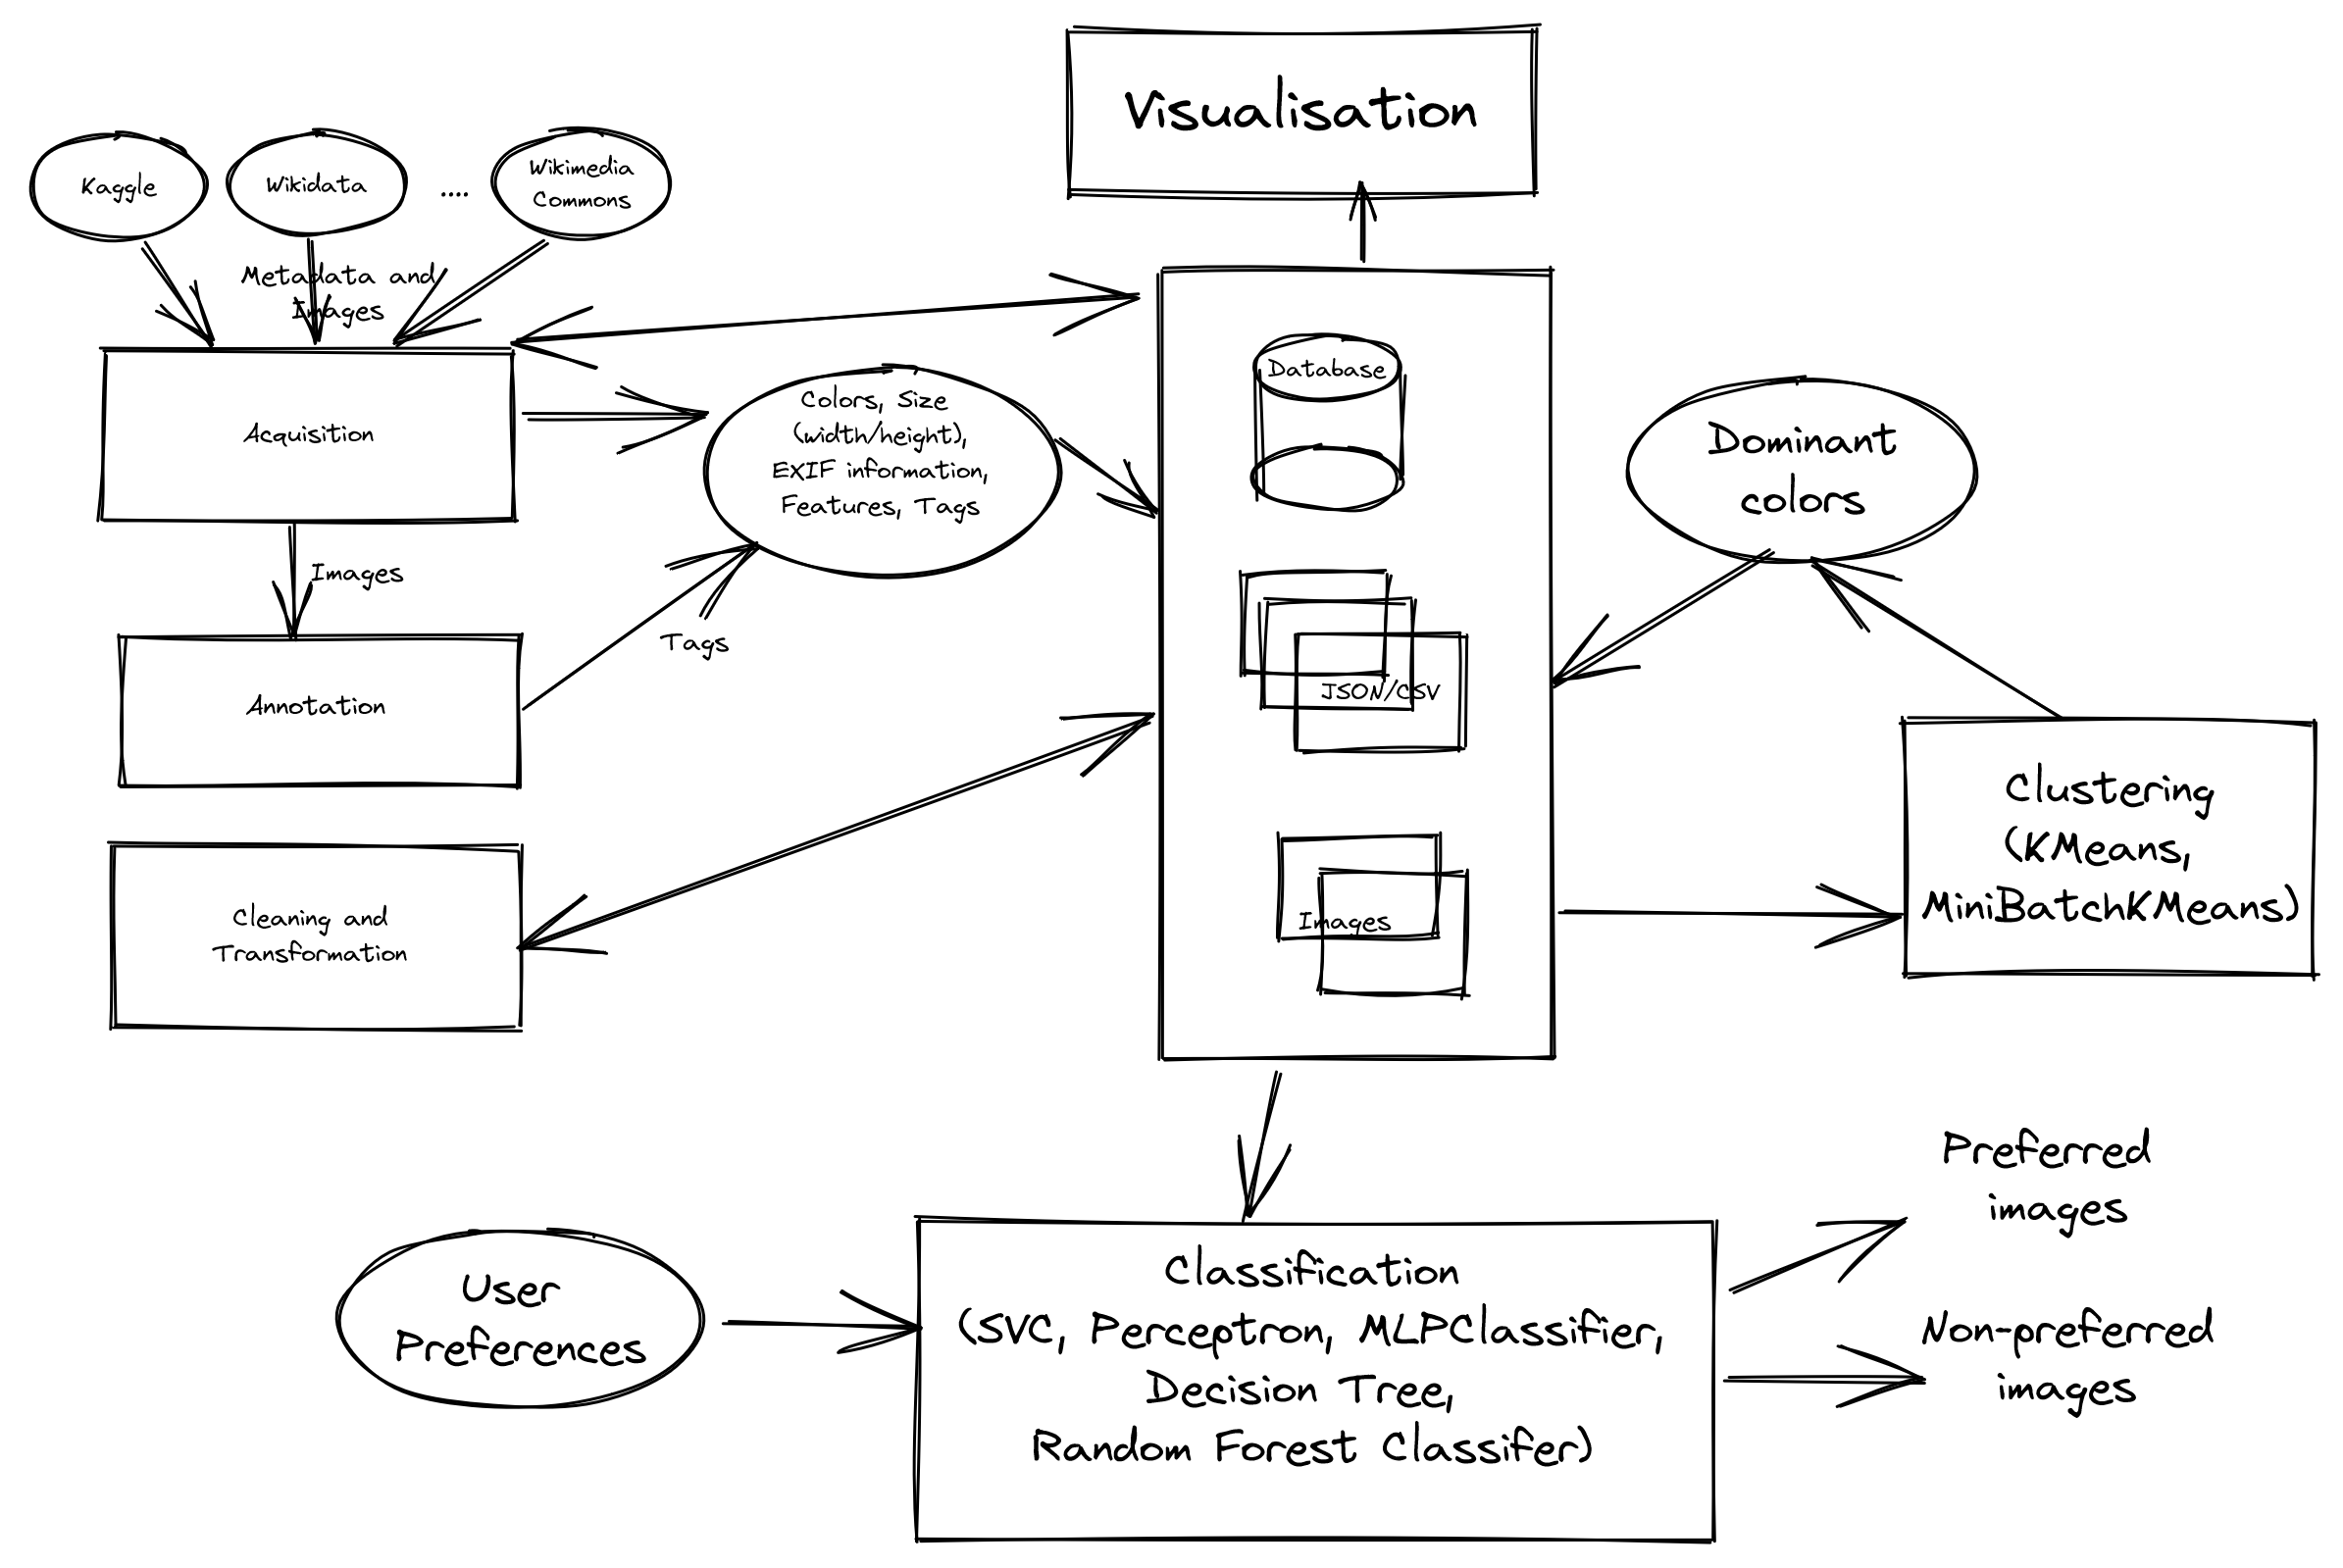
\includegraphics[width=0.8 \textwidth]{img/targeted_archi}
        \caption{Targeted architecture}
        \label{fig:targeted_architecture}
    \end{figure}

    \subsection{actual architecture}\label{subsec:actual_architecture}

    \begin{figure}[htbp]
        \centering
        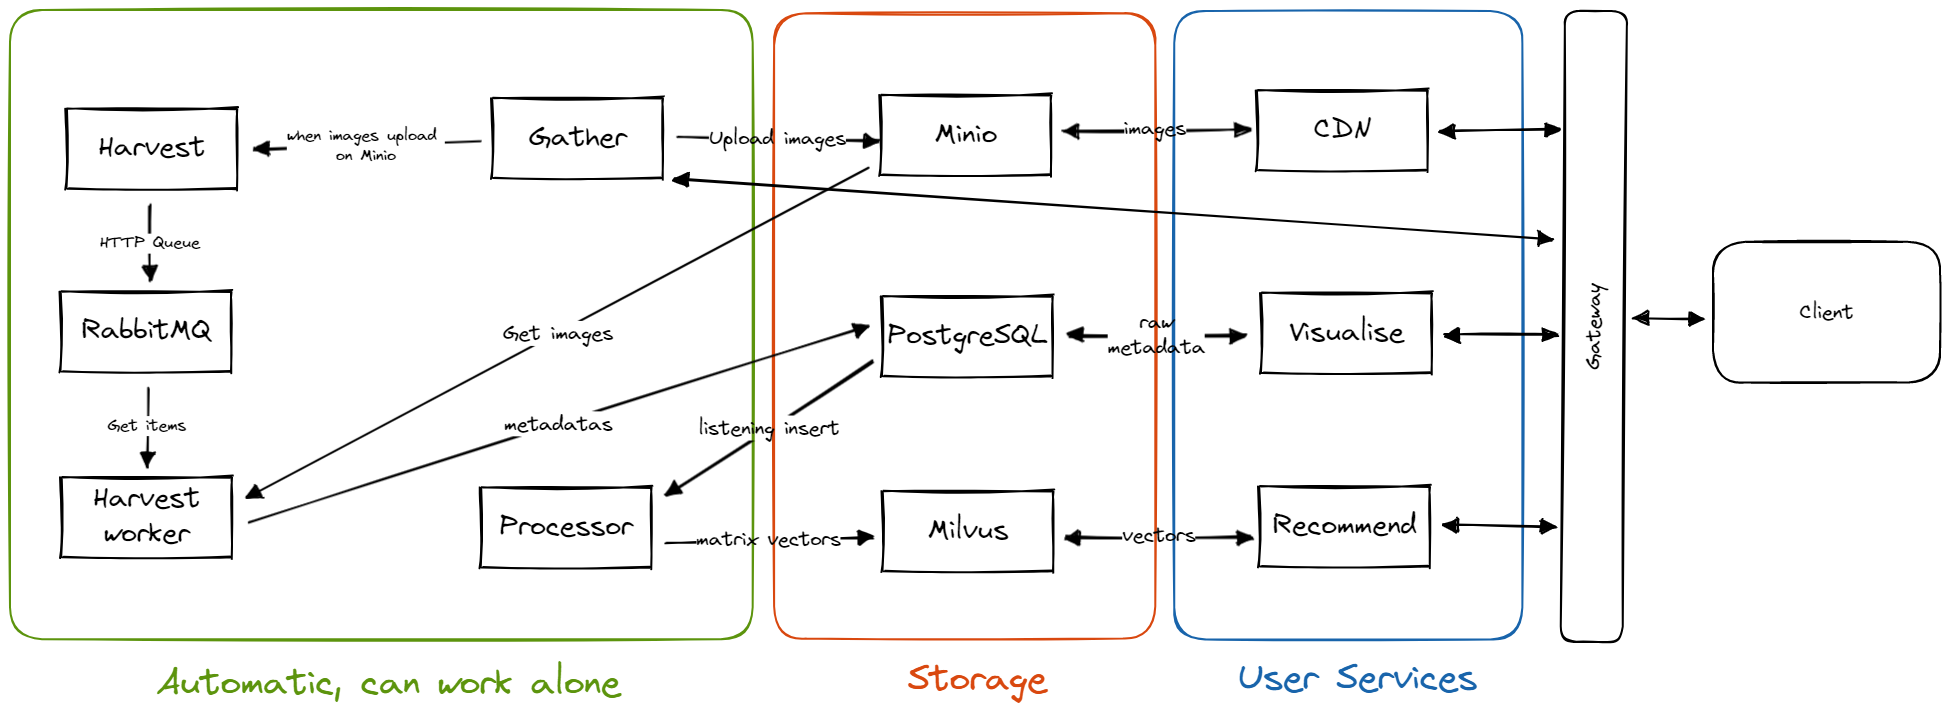
\includegraphics[width=1.2\textwidth]{img/actual_architecture}
        \caption{Actual architecture}
        \label{fig:actual_architecture}
    \end{figure}

    \newpage

    \subsection{Graphs}\label{subsec:graphs}

    \subsubsection{static sizes}\label{subsubsec:static_sizes}

    \begin{figure}[htbp]
        \centering
        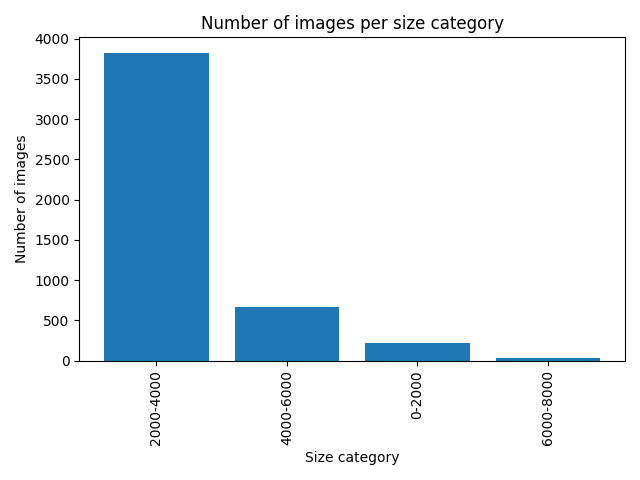
\includegraphics[width=0.7 \textwidth]{img/size_static}
        \caption{Sizes}
        \label{fig:static_sizes}
    \end{figure}

    \subsubsection{dynamic sizes}\label{subsubsec:dynamic_sizes}

    \begin{figure}[htbp]
        \centering
        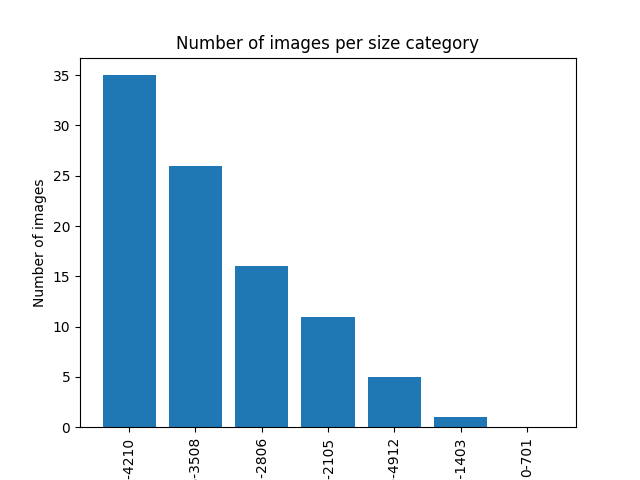
\includegraphics[width=0.65 \textwidth]{img/size_dynamic}
        \caption{Sizes}
        \label{fig:dynamic_sizes}
    \end{figure}

    \newpage


    \subsubsection{Top years}\label{subsubsec:top_years}

    \begin{figure}[htbp]
        \centering
        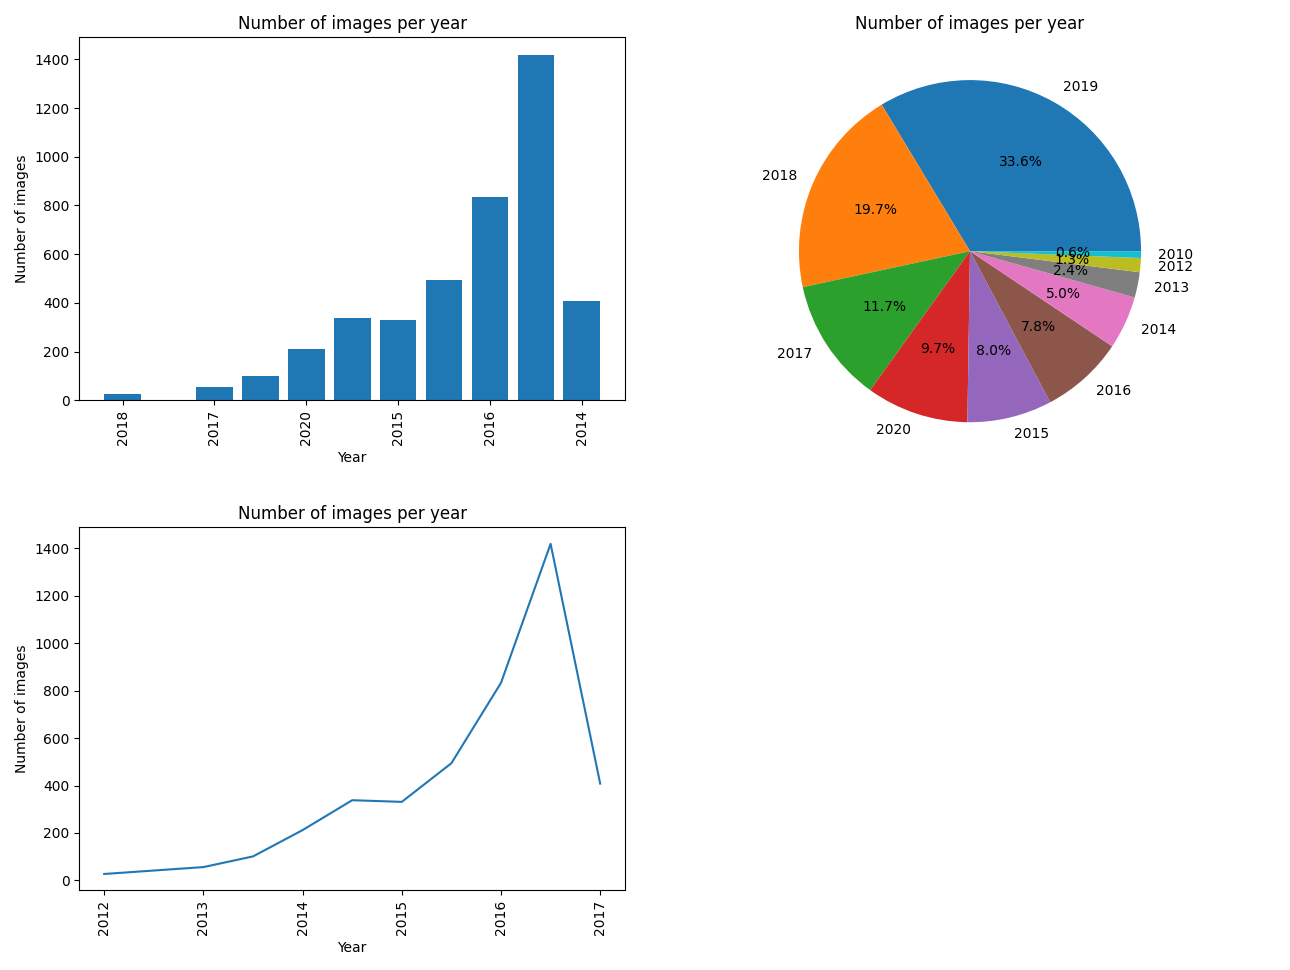
\includegraphics[width=0.65 \textwidth]{img/year}
        \caption{Top years}
        \label{fig:top_years}
    \end{figure}

    \subsubsection{Top altitudes}\label{subsubsec:top_altitudes}

    \begin{figure}[htbp]
        \centering
        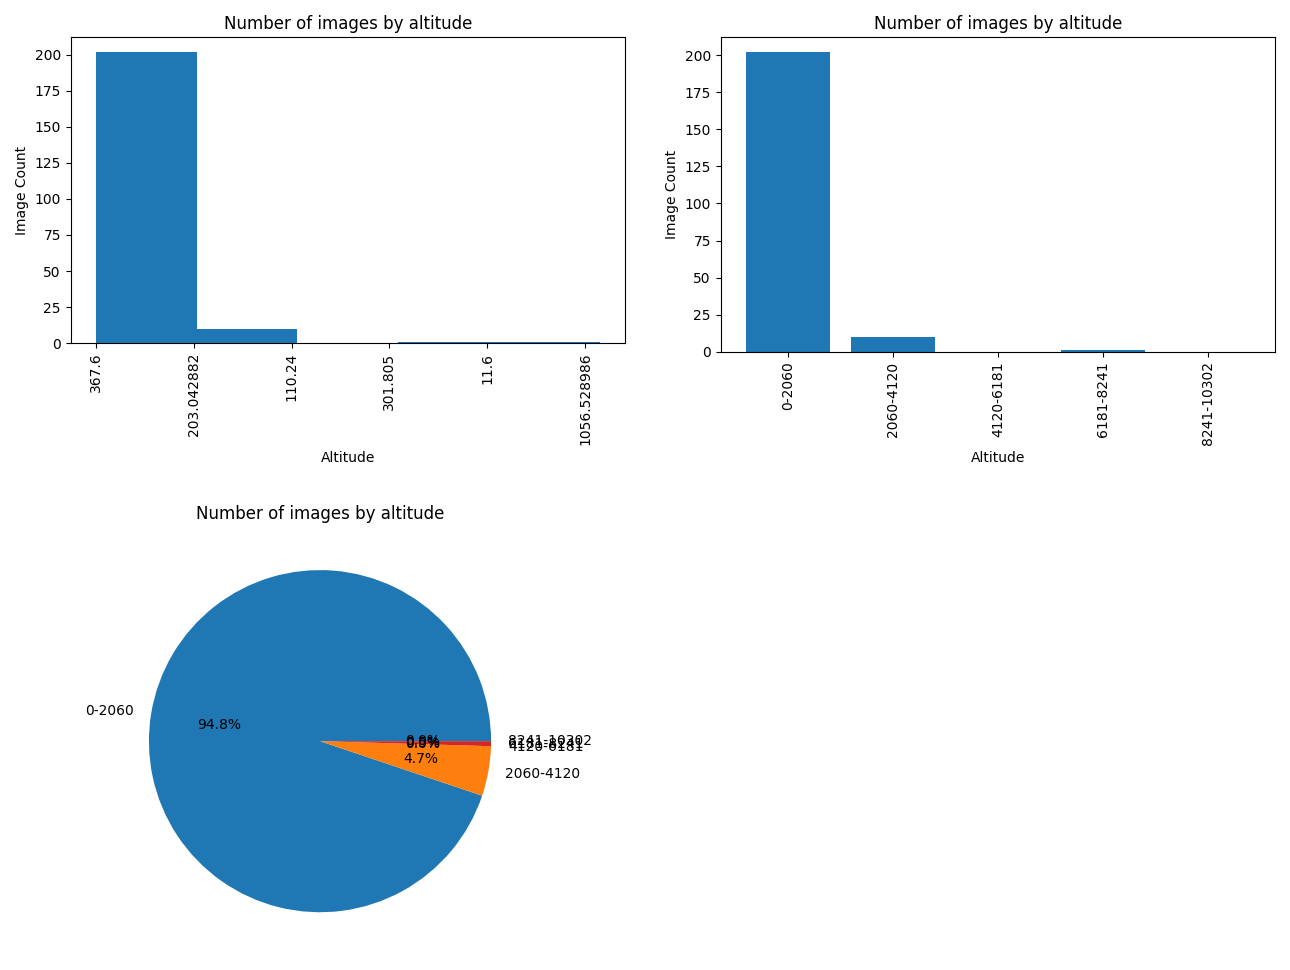
\includegraphics[width=0.65 \textwidth]{img/altitude}
        \caption{Top altitudes}
        \label{fig:top_altitudes}
    \end{figure}

    \newpage

    \subsubsection{Top countries}\label{subsubsec:top_countries}

    \begin{figure}[htbp]
        \centering
        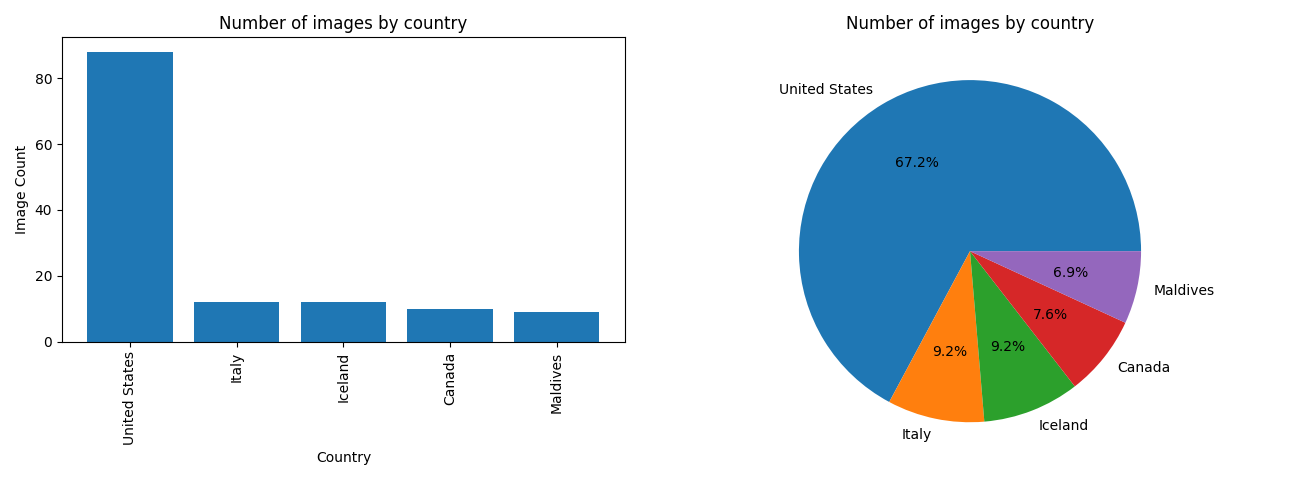
\includegraphics[width=1.1 \textwidth]{img/country}
        \caption{Top countries}
        \label{fig:top_countries}
    \end{figure}

    \subsubsection{Map}\label{subsubsec:map}

    \begin{figure}[htbp]
        \centering
        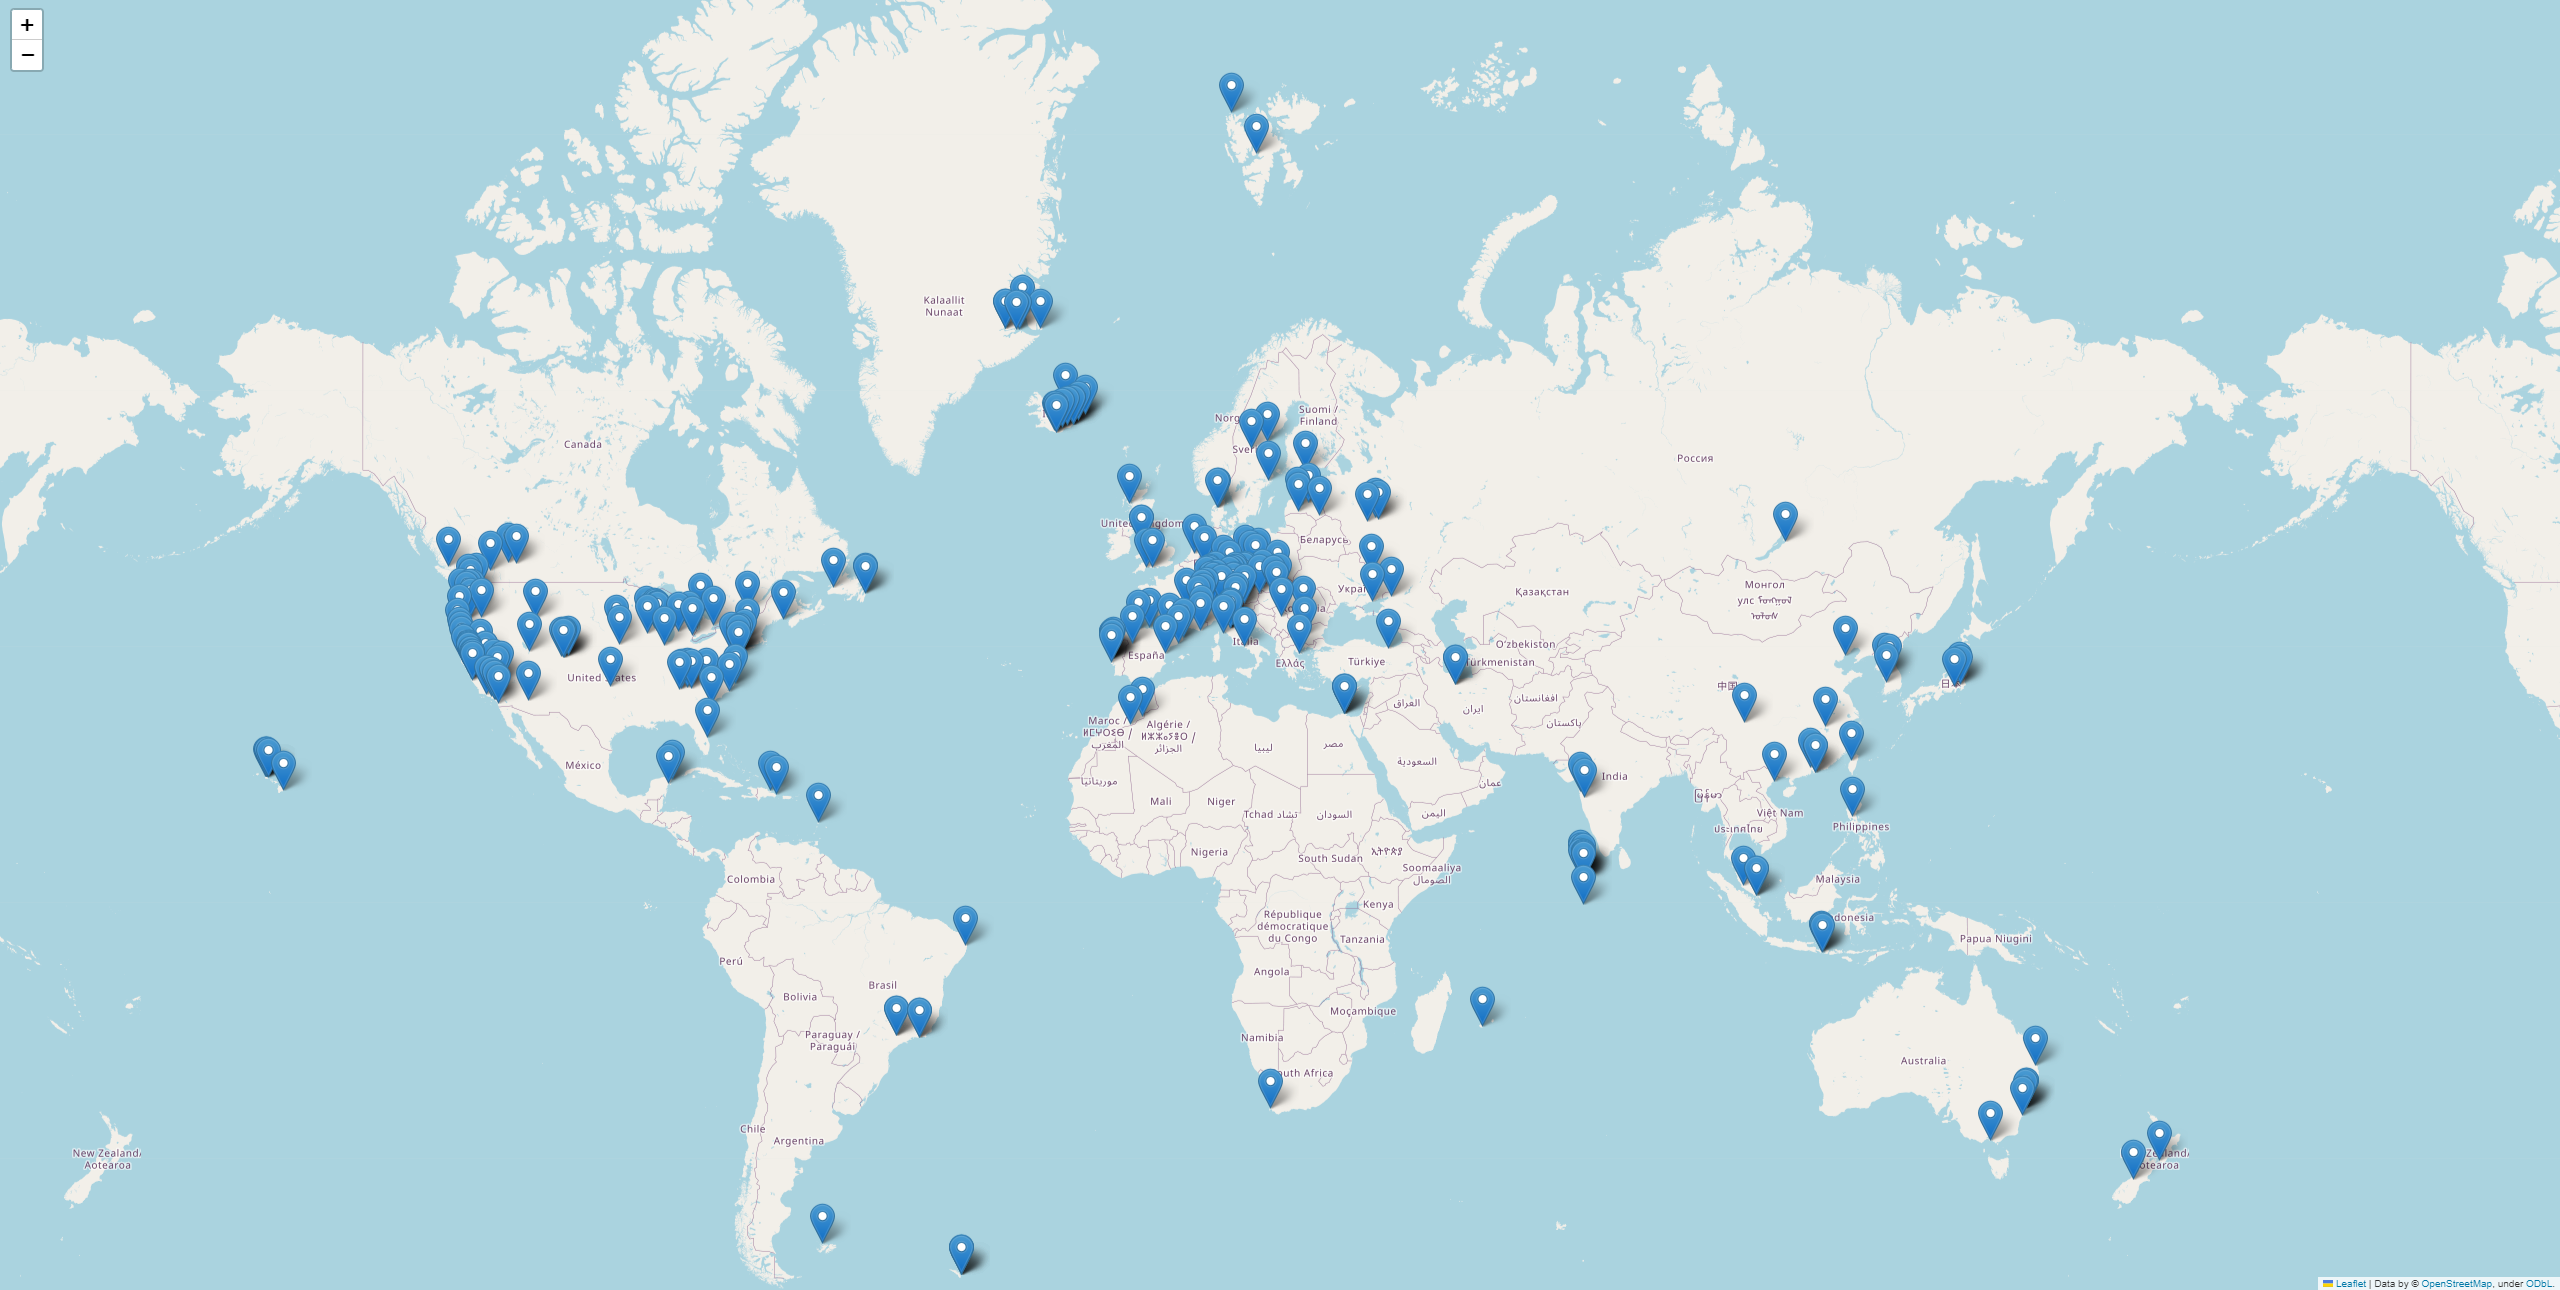
\includegraphics[width=1.1 \textwidth]{img/map}
        \caption{Map}
        \label{fig:map}
    \end{figure}

    \newpage

    \subsubsection{Dominant colors}\label{subsubsec:dominant_colors}

    \begin{figure}[htbp]
        \centering
        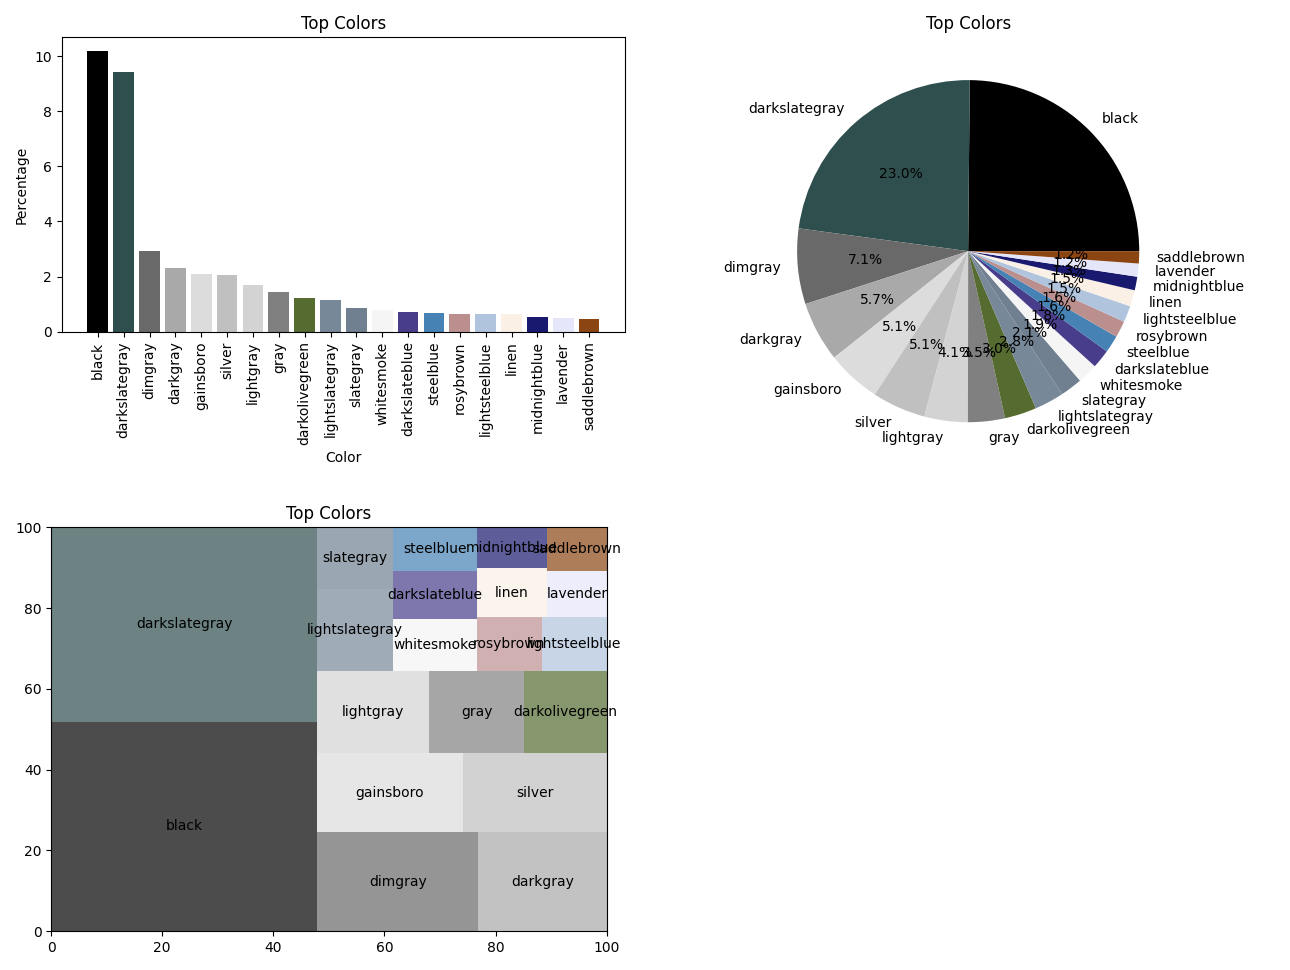
\includegraphics[width=0.9 \textwidth]{img/dominant_color}
        \caption{Top colors}
        \label{fig:dominant_colors}

    \end{figure}

    \subsubsection{Top brands}\label{subsubsec:top_brands}

    \begin{figure}[htbp]
        \centering
        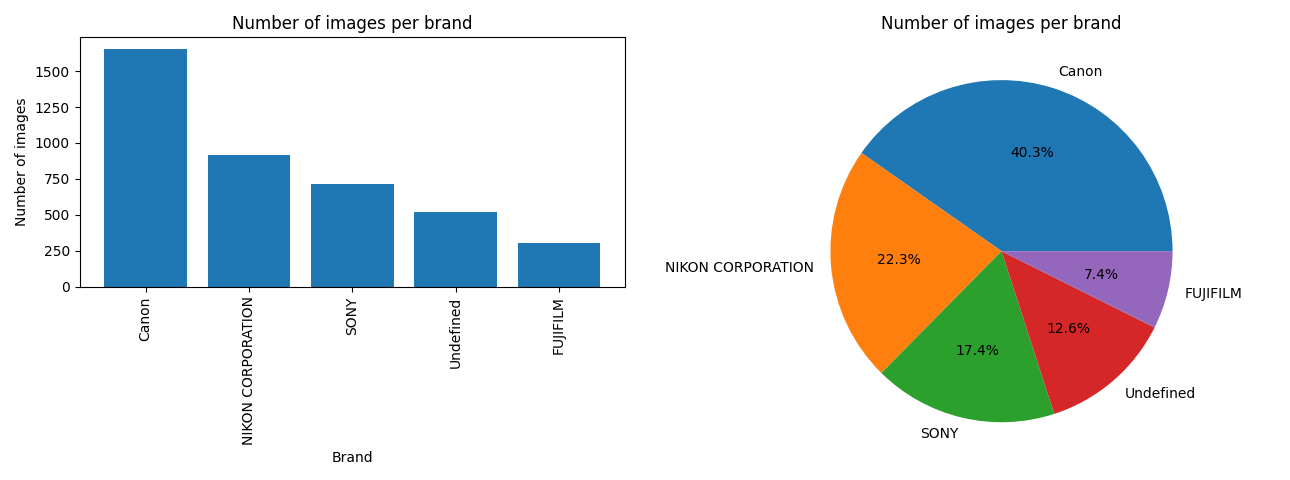
\includegraphics[width=0.8 \textwidth]{img/brand}
        \caption{Top brands}
        \label{fig:top_brands}
    \end{figure}

    \newpage

    \subsubsection{Top tags}\label{subsubsec:top_tags}

    \begin{figure}[htbp]
        \centering
        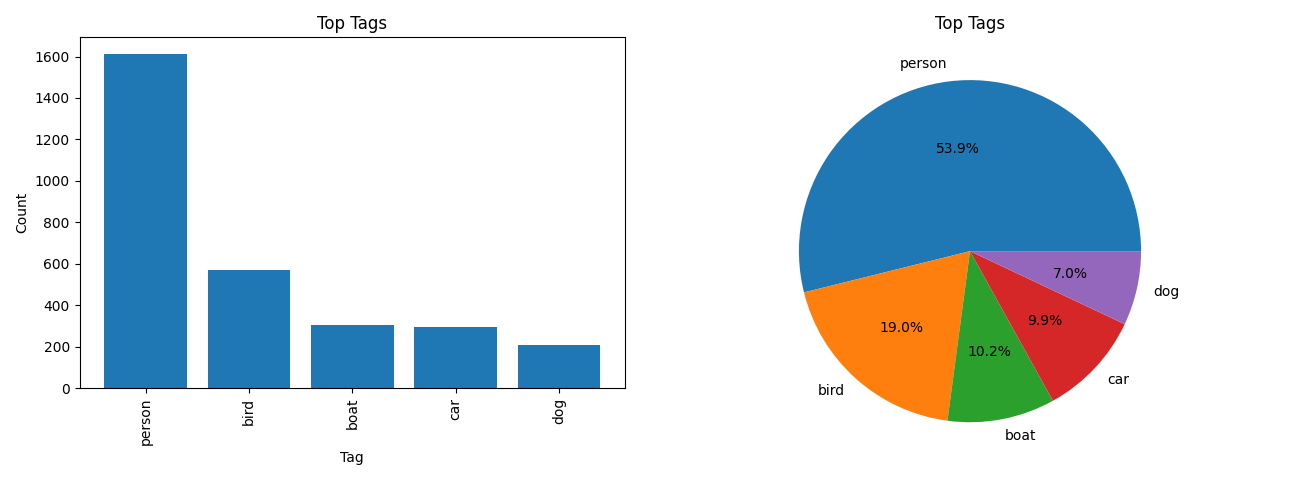
\includegraphics[width=0.85 \textwidth]{img/tags}
        \caption{Top tags}
        \label{fig:top_tags}
    \end{figure}

    \subsubsection{Dendrogram}\label{subsubsec:dendrogram}

    \begin{figure}[htbp]
        \centering
        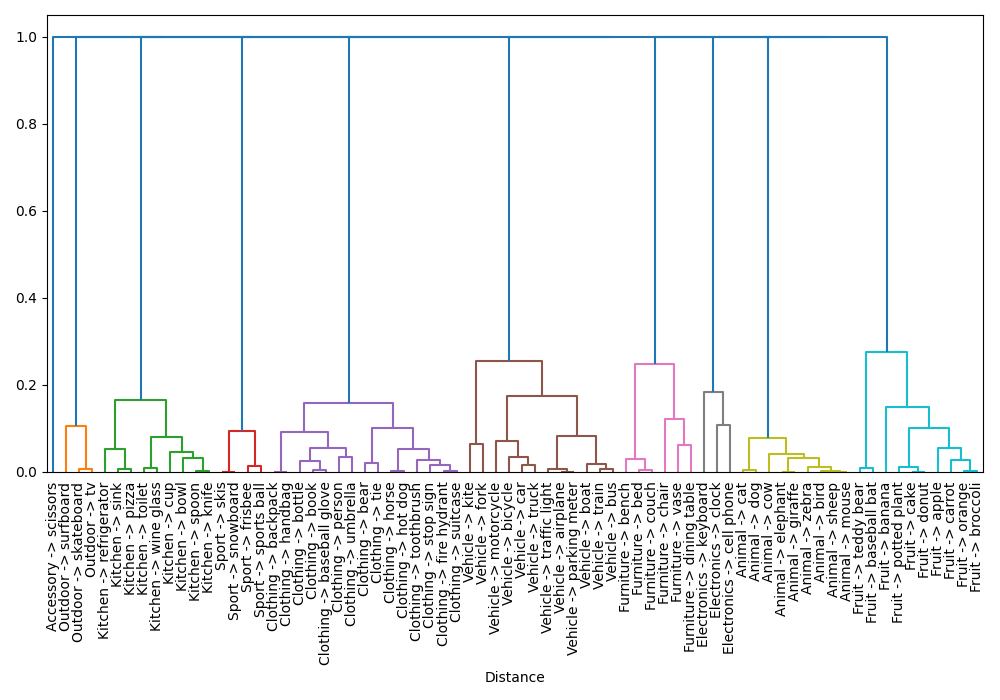
\includegraphics[width=1 \textwidth]{img/dendrogram}
        \caption{Dendrogram}
        \label{fig:dendrogram}
    \end{figure}

\end{document}



